\documentclass[12pt]{article}
\usepackage{float}
\usepackage{gensymb}
\usepackage{amsmath}
\usepackage{graphics}                        
\usepackage{graphicx}                    
\graphicspath{{storage/self/primary/Download/asgnt6/fig}}        
\graphicspath{{storage/self/primary/Download/asgnt6/table}}
\providecommand{\brak}[1]{\ensuremath{\left(#1\right)}}
\providecommand{\myvec}[1]{\ensuremath{\begin{pmatrix}#1\end{pmatrix}}}
\providecommand{\mydet}[1]{\ensuremath{\begin{vmatrix}#1\end{vmatrix}}}
\providecommand{\norm}[1]{\ensuremath{\lvert|#1\rvert|}}
\let\vec\mathbf
\begin{document}
\title{\textbf{9.10.4.3}}
\date{}
\maketitle
\textbf{Question :} If two equal chords of a circle intersect within the circle,prove that the line joining the point of intersection to the centre makes equal angles with the chords.

\textbf{Solution :}

\begin{table}[H]
    \centering
      \begin{tabular}{|c|c|c|}
    \hline
    \textbf{Input Parameters} &\textbf{Description} &\textbf{Value} \\
    \hline
     $\vec{O}$& Center(at origin)&$\vec{0}$\\
     \hline
 $r$ & Radius &1\\
 \hline
 $\theta$&-&$100\degree$\\
 \hline
 $\alpha$&-&$165.4\degree$\\
 \hline
 $\beta$&-&$5\degree$\\
 \hline
  \end{tabular}

    \caption{Table of input parameters}
    \label{tab:tab:9.10.4.3.1}
\end{table}

\begin{table}[H]
    \centering
\begin{tabular}{|c|c|c|}
    \hline
        \textbf{Output Parameters} &\textbf{Description} &\textbf{Value} \\
\hline
          $\vec{Q}$ & Point &$\myvec{\cos{\theta_1}\\\sin{\theta_1}}$\\
          \hline
          $\vec{P}$ & Point &$\myvec{\cos{\theta_2}\\\sin{\theta_2}}$ \\
         \hline
          $\vec{R}$ & Point &$\myvec{\cos{\theta_3}\\sin{\theta_3}}$ \\
         \hline
    \end{tabular}


\caption{Table of output parameters}
    \label{tab:tab:9.10.4.3.2}
\end{table}

\begin{align}
  \cos{\angle RQS}&=\frac{\vec{\brak{R-Q}}^{\top}\vec{\brak{Q-S}}}{\vec{\norm{R-Q}\norm{Q-S}}}\\
  &=\cos{\frac{\theta_3-\theta_4}{2}}\\
   \cos{\angle PSQ}&=\frac{\vec{\brak{P-S}}^{\top}\vec{\brak{S-Q}}}{\vec{\norm{P-S}\norm{S-Q}}}\\
  &=\cos{\frac{\theta_1-\theta_2}{2}}\\
   \cos{\angle RQS}&=\cos{\angle PSQ}\\
   or,\theta_1&=\theta_2-\theta_3+\theta_4\\
   &=-180\degree
  \end{align}
The equation of $PQ$ and $RS$ is obtained by
\begin{align}
  \vec{n_1}^{\top}\vec{\brak{x-P}}=0\\
  \vec{n_2}^{\top}\vec{\brak{x-R}}=0\\
  or,\vec{n_1}=\myvec{\sin{\theta_2}-\sin{\theta_1}\\\cos{\theta_1}-\cos{\theta_2}}\\
  or,\vec{n_2}=\myvec{\sin{\theta_4}-\sin{\theta_3}\\\cos{\theta_3}-\cos{\theta_4}}\\
 \end{align}
  The value of the point of the intersection is
\begin{align}
    \myvec{\vec{n_1}^{\top}\\\vec{n_2}^{\top}}\vec{X}&=\myvec{\vec{n_1}^{\top}\vec{P}\\\vec{n_2}^{\top}\vec{R}}
    \end{align}
\begin{multline}
    \vec{X}=\frac{1}{\mydet{\cos{\theta_3}-\cos{\theta_4}&\cos{\theta_2}-\cos{\theta_1}\\\sin{\theta_3}-\sin{\theta_4}&\sin{\theta_2}-\sin{\theta_1}}}\\\times
    \myvec{\cos{\theta_3}-\cos{\theta_4}&\cos{\theta_2}-\cos{\theta_1}\\\sin{\theta_3}-\sin{\theta_4}&\sin{\theta_2}-\sin{\theta_1}}\myvec{\sin{\theta_2-\theta_1}\\\sin{\theta_4-\theta_3}}\\
\end{multline}
    \begin{align}
        or,\vec{T} &= \myvec{0\\-0.45}\\
\cos{\angle OTP} &= \frac{\brak{\vec{T-P}}^{\top}\brak{\vec{O-T}}}{\vec{\norm{T-P}\norm{T-O}}}\\
or, \angle OTP&= 66\degree
\end{align}
Similarly,
\begin{align}
   \cos{\angle OTR} &= \frac{\brak{\vec{T-R}}^{\top}\brak{\vec{T-O}}}{\vec{\norm{T-R}\norm{T-O}}}\\
or, \angle OTR&= 66\degree \\
So,\angle OTP &= \angle OTR \brak{proved}
\end{align}

 

\begin{figure}[H]                            
\centering
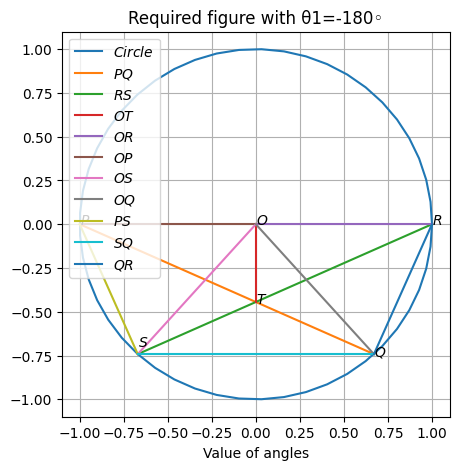
\includegraphics[width=\columnwidth]{fig/9.10.4.3.png}                            
\caption{}                              
\label{fig:9.10.4.3}
\end{figure}
\end{document}

